%! suppress = Unicode
\documentclass[12pt, a4paper]{article}

\usepackage[czech,shorthands=off]{babel}
\usepackage{lmodern}
\usepackage[utf8]{inputenc}
\usepackage[T1]{fontenc}
\usepackage[pdftex]{graphicx}
\usepackage{amsmath}
\usepackage[hidelinks,unicode]{hyperref}
\usepackage{float}
\usepackage{listings}
\usepackage{tikz}
\usepackage{xcolor}
\usepackage{tabularx}
\usepackage[final]{pdfpages}
\usepackage{syntax}
\usepackage{listings}


\definecolor{mauve}{rgb}{0.58,0,0.82}
\usetikzlibrary{shapes,positioning,matrix,arrows}

\newcommand{\img}[1]{(viz obr. \ref{#1})}

\definecolor{pblue}{rgb}{0.13,0.13,1}
\definecolor{pgreen}{rgb}{0,0.5,0}
\definecolor{pred}{rgb}{0.9,0,0}
\definecolor{pgrey}{rgb}{0.46,0.45,0.48}

\usepackage[sorting=nyt,style=ieee]{biblatex}
\addbibresource{literatura.bib}

\lstdefinestyle{sharpc}{language=[Sharp]C, frame=lr, rulecolor=\color{blue!80!black}}

\lstdefinestyle{flex}{
    frame=tb,
    aboveskip=3mm,
    belowskip=3mm,
    showstringspaces=false,
    columns=flexible,
    basicstyle={\small\ttfamily},
    numbers=none,
    numberstyle=\tiny\color{black},
    keywordstyle=\color{black},
    commentstyle=\color{black},
    stringstyle=\color{black},
    breaklines=true,
    breakatwhitespace=true,
    tabsize=3
}
\lstset{style=sharpc}
\lstset{
    frame=tb,
    language=XML,
    aboveskip=3mm,
    belowskip=3mm,
    showstringspaces=false,
    columns=flexible,
    basicstyle={\small\ttfamily},
    numbers=none,
    numberstyle=\tiny\color{gray},
    keywordstyle=\color{blue},
    commentstyle=\color{pgreen},
    stringstyle=\color{mauve},
    breaklines=true,
    breakatwhitespace=true,
    tabsize=3
}


\let\oldsection\section\renewcommand\section{\clearpage\oldsection}

\begin{document}
    % this has to be placed here, after document has been created
    % \counterwithout{lstlisting}{chapter}
    \renewcommand{\lstlistingname}{Ukázka kódu}
    \renewcommand{\lstlistlistingname}{Seznam ukázek kódu}
    \begin{titlepage}

        \centering

        \vspace*{\baselineskip}
        \begin{figure}[H]
            \centering
            
\includegraphics[width=7cm]{img/fav-logo.jpg}
        \end{figure}

        \vspace*{1\baselineskip}

        \vspace{0.75\baselineskip}

        \vspace{0.5\baselineskip}
        {Semestrální práce z předmětu KIV/NET}

        {\LARGE\sc Aplikace pro sledování obchodního portfólia s kryptoměnami \\}

        \vspace{4\baselineskip}

        \vspace{0.5\baselineskip}

        {\sc\Large Stanislav Král \\}
        \vspace{0.5\baselineskip}
        {A20N0091P}

        \vfill

        {\sc Západočeská univerzita v Plzni\\
        Fakulta aplikovaných věd}

    \end{titlepage}


    % TOC
    \tableofcontents
    \pagebreak


    \section{Zadání práce}
    Zadáním práce je vytvořit aplikaci určenou ke sledování obchodního portfólia s kryptoměnami pomocí frameworku .NET 5.0, kdy aplikace bude nabízet grafické rozhraní pro její ovládání. Aplikace musí splňovat následující body:

    \begin{itemize}
        \item možnost vytvořit portfólia, do kterých budou členěněny jednotlivé transakce (jedno portfólio může obsahovat pouze transakce v jedné fiat měně)
        \item jednotlivé transakce budou obsahovat informaci o nákupní či prodejní ceně za jednu minci kryptoměny, počet mincí, kterých se obchod týkal, datum uskutečnění obchodu a poplatek za jeho zprostředkování
        \item možnost zobrazit si celkový zisk či ztrátu portfólia
        \item možnost zobrazit si zisk či ztrátu na úrovni jednotlivých transakcí
        \item možnost zobrazit si procentuální složení daného portfólia
        \item možnost získat aktuální kurz vybrané kryptoměny ze zdroje dostupného přes veřejně dostupné REST API
        \item vhodně navržená architektura umožující možnost jednoduchou výměnu datové vrstvy či zdroje aktuálního kurzu
    \end{itemize}


    \section{Sledování obchodního portfólia s kryptoměnami}

    Obchodování kryptoměň spočívá v nákupu a prodeji kryptoměn na burzách za účelem zisku, kdy obchodník chce prodat kryptoměny za vyšší částku než je nakoupil. Je typické, že takový obchodník provádí velké množství obchodů (až několik týdně) a i přesto, že burzy s kryptoměnami sice poskytují přehled historie uskutečněných transakcí, tak tento přehled nebývá často dostatečně obsáhlý a některé informace, jako například zisk či ztráta, se v něm nezobrazují. Dále je také časté, že obchodníci používají k obchodování více než jednu burzu, a tak vzniká potřeba nějaké služby či aplikace, ve které by byly transakce ze všech burz uložené, a která by nabízela jednoduché a společné rozhraní pro všechny burzy. Od takové služby je vyžadovaný i kvalitní přehled zobrazující aktuální výkon obchodování a celkovou hodnotu výdělku či ztráty. Mezi nejpopulárnější kryptoměnové burzy patří například \textit{Coinbase} či \textit{Binance}.

    Za předpokladu existence takové aplikace by jejím dalším využitím, jelikož sdružuje transakce ze všech burz, bylo použití při vyplňování daňového přiznání, kdy je velmi výhodné, že aplikace zobrazuje všechny obchodníkovy transakce včetně zisku či ztráty.

    Aplikací, které se zaměřují na sledování obchodního portfólia s kryptoměnami existuje několik, kdy mezi ty nejpoužívanější patří Blockfolio\cite{blockfolio2021} (Android a iOS), Delta\cite{delta2021} (Android a iOS) a Moonitor\cite{moonitor2021} (macOS, Windows a Linux). Tyto aplikace splňují požadavek přehledného zobrazení výnosnosti obchodování i na úrovni jednotlivých transakcí, avšak během jejich používání můžou často vzniknout nové požadavky specifické danému uživateli, jako například možnost importu transakcí z API nějaké méně známé burzy či jiný výpočet celkového zisku portfólia, které do aplikace pravděpodobně nikdy nebudou zapracovány. Řešením pro technicky zdatné uživatele by bylo si takovou aplikaci navrhnout a napragramovat, avšak vytváření architektury a základní logiky pro správu a sledování portfólia (zádávní transakcí a jejich přehled) pro ně může být časově náročné a tudíž odrazující.

    \begin{figure}[!ht]
        \centering
        {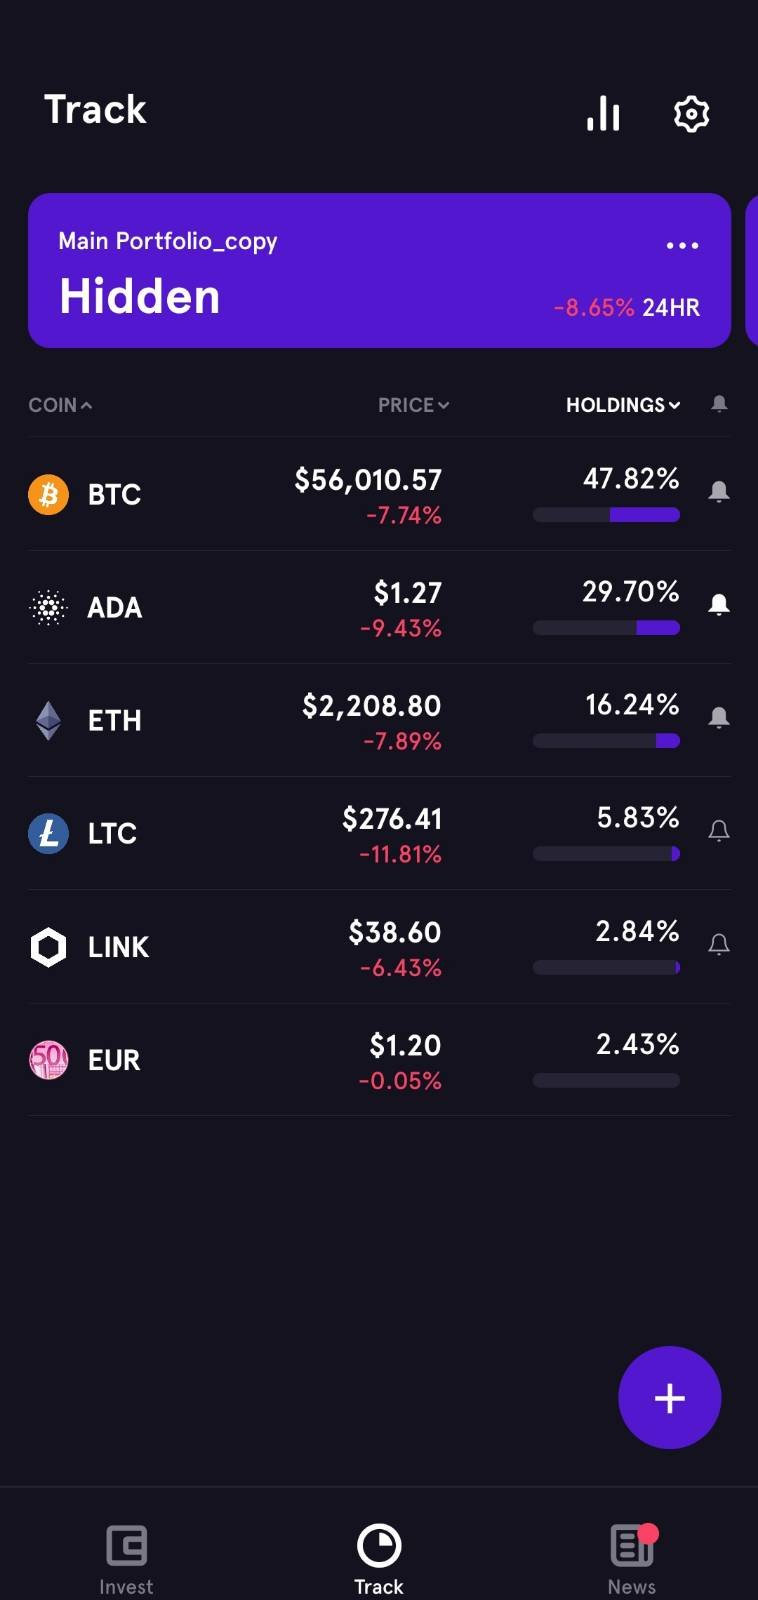
\includegraphics[width=5.5cm]{img/blockfolio.png}}
        \caption{Mobilní aplikace Blockfolio umožňující sledovat kryptoměnové portfólio}
        \label{fig:simple-vrp-czech}
    \end{figure}


    \section{Analýza}
    
    \subsection{Datový zdroj s aktuálním kurzem kryptoměn}

    Pro vývoj aplikace určené ke sledování obchodního portfólia s kryptoměnami je třeba nalézt vhodný zdroj dat, který bude využíván k získávání aktuálního kurzu sledovaných kryptoměn. Mezi hlavní požadavky na takový datový zdroj je jeho dostupnostie jednoduchost rozhraní a množina podporovaných kurzů. Ideálním zdrojem je tedy takový zdroj, který poskytuje aktuální i historický kurz na všech burzách prostřednictvím REST API bez nutnosti registrace.

    \subsubsection{Webový zdroj CoinGecko}
    Aktuální i historický kurz drtivé většiny všech existujících kryptoměn bez nutnosti registrace nabízí pomocí REST rozhraní webová služba CoinGecko\cite{coingecko2021}. Jediným omezením tohoto API je počet provedených požadavků za minutu, který je stanoven na 100, což je pro aplikaci určenou ke sledování kryptoměnového portfólia více než dostačující.

    \begin{lstlisting}
\$ curl -X GET "https://api.coingecko.com/api/v3/simple/price?ids=bitcoin&vs_currencies=usd" -H  "accept: application/json"

{
  "bitcoin": {
    "usd": 56224
  }
}
    \end{lstlisting}

    \subsection{Výběr databáze pro implementaci datové vrstvy aplikace}

    Jelikož vytvářená aplikace není určená pro použití vícero uživateli najednou, ale pouze pro jednoho uživatele na jednom zařízení, tak pro ukládání dat aplikace je vhodná lokální databáze.

    V úvahu připadá ukládat portfólia a transakce ve formátu JSON či XML přímo na souborový systém, ale z důvodu relace M:N mezi portfólii a kryptoměnami nejsou tyto typy databází příliš vhodné. Jako lepší volba tedy jeví nějaká relační databáze, např. SQLite, která je často používána při tvorbě desktopových aplikací a ukládá se ve formě jednoho souboru na souborový systém zařízení.

    \section{Popis architektury vytvořené aplikace}

    \subsection{Databázová vrstva}
    Ve vytvořené aplikaci je datová vrstva implementována pomocí tzv. \textit{repozitářů}, kdy každý repozitář představuje perzistentní úložiště dané entity, do kterého lze zapisovat a následně z něj číst.

    Kontrakt generického rozhraní repozitáře se skládá z následujících definic metod:
    \begin{itemize}
        \item \texttt{public int Add(T entry)} -- přidá daný objekt do perzistentního úložiště a vrátí vygenerované ID
        \item \texttt{public T Get(int id)} -- vyhledá a případně vrátí objekt z perzistentního úložiště dle předaného identifikátoru \texttt{id}
        \item \texttt{List<T> GetAll()} -- vyhledá a případně vrátí seznam všech objektů z perzistentního úložiště
        \item \texttt{public bool Update(T entry)} -- nahraje do perzistentního úložiště aktualizovanou verzi objektu, který se zde již nachází. Vrátí \texttt{true}, pokud aktualizace proběhla úspěšně nebo \texttt{false}, pokud během této operace došlo k nějaké chybě.
        \item \texttt{public bool Delete(T entry)} -- smaže předaný objekt z úložiště a vrátí \texttt{true}, pokud smazání proběhlo úspěšně nebo \texttt{false}, pokud během této operace došlo k nějaké chybě.

    \end{itemize}

    \noindent Ve vytvořené aplikaci jsou definovány následující repozitáře:
    \begin{itemize}
        \item \texttt{IPortfolioRepository} -- úložiště objektů představujících jednotlivá portfólia spravované v aplikaci
        \item \texttt{IPortfolioEntryRepository} -- úložiště objektů představujících položky existujících portfólií
        \item \texttt{IMarketOrderRepository} -- úložiště objektů představujících uskutečněné obchody dané položky portfólia
    \end{itemize}

    \subsubsection{Generování SQL dotazů}
    K jednoduchému a intuitivnímu generování SQL dotazů je použita knihovna \textbf{SqlKata Query Builder}\footnote{\url{https://github.com/sqlkata/querybuilder}}, kdy lze SQL dotazy vytvářet pomocí řetězení volání metod poskytovaných touto knihovnou.

    \begin{lstlisting}[language=Java, caption={Příklad generování SQL dotazu pro výběr všech transakcí dané položky portfólia pomocí knihovny SqlKata Query Builder.},captionpos=b, label={lst:sm-showcase}]
Db.Get().Query("orders").Where("portfolio_entry_id", portfolioEntryId).Get()
    \end{lstlisting}

    Tato knihovna přímo umožňuje nad předaným databázovým spojením vygenerovaný SQL dotaz přímo vykonat, kdy k této činnosti využívá knihovnu \textbf{Dapper}\footnote{\url{https://github.com/DapperLib/Dapper}}.
    Výsledkem metod bez specifikování typu pro vykonání generovaných dotazů jsou objekty typu \texttt{dynamic}, které je třeba mapovat na instance tříd dle modelu entity se kterou pracujeme.

    \begin{lstlisting}[language=Java,caption={Příklad mapování objektu typu \texttt{dynamic} na instanci třídy \texttt{Portfolio}.},captionpos=b, label={lst:sm-mapping}]
public override Portfolio FromRow(dynamic d) =>
            new Portfolio((string) d.name, (string) d.description, (Currency) d.currency_code, (int) d.id);
    \end{lstlisting}

    Jelikož velká část kódu pro implementaci metod repozitáře je pro všechny možné typy stejná, tak je tato část kódu sdílena pomocí abstraktní třídy \texttt{SqlKataRepository}. Implementace pro konkrétní třídy modelu musí akorát implementovat kód pro vytvoření instance dané třídy z objektu typu \texttt{dynamic} a naopak. V aplikaci se nachází implementace \texttt{SqlKataPortfolioRepository}, \texttt{SqlKataPortfolioEntryRepository} a \texttt{SqlKataMarketOrderRepository}.
    
    \subsection{Služba \texttt{IPortfolioService}}
    Tato služba poskytuje rozhraní pro správu portfólií v perzistentním úložišti.
    Umožňuje vytvořit a přidat nové portfólio do repozitáře na základě jeho atributů předaných pomocí parametrů.
    Dále také poskytuje metodu pro smazání portfólia, která smaže i všechny jeho položky.
    
    \subsection{Služba \texttt{IPortfolioEntryService}}
    Velmi podobně jako služba \texttt{IPortfolioService}, tato služba poskytuje rozhraní pro správu položek portfólií v perzistentním úložišti.
    Kromě vytvoření a přidání nových položek na základě parametrů také nabízí metodu pro její smazání, která smažá i všechny transakce, které k ní byly přiřazeny. 
    Dále disponuje metodou pro výběr všech položek, které patří do vybraného portfólia.
    
    \subsection{Služba \texttt{IMarketOrderService}}
    Rozhraní pro správu transakcí v perzistentním úložišti poskytuje právě tato služba, kdy poskytuje i metodu pro vyhledání všech transakcí patřících do vybrané položky portfólia.

    \subsection{Napojení na online datový zdroj kurzů kryptoměn}
    Aby aplikace mohla zobrazovat nejaktuálnější výnosnost investicí, tak potřebuje být schopna získávat data z datového zdroje kurzů kryptoměn.
    Pro tyto účely slouží obecné rozhraní \texttt{ICryptoStatsSource}, které definuje následující metody:

    \begin{itemize}
        \item \texttt{GetMarketEntries(string currency, params string[] ids)} -- stáhne nejaktuálnější informace o vybraných kryptoměnách, kdy údaje o cenách jsou ve měně vybrané pomocí parametru \texttt{currency}.
        Mezi stahované informace patří například zkratka kryptoměny, její název, aktuální hodnota či tržní kapitalizace.
        \item \texttt{GetAvailableCryptocurrencies()} -- stáhne seznam kryptoměn, na které se může volající datového zdroje tázat.
        V seznamu dostupných kryptoměn je u každé informace o jejím názvu, zkratce a identifikátoru.
    \end{itemize}

    Ve vytvořené aplikaci se nachází implementace \texttt{CoingeckoSource}, která k získávání informací o kryptoměnách používá REST API rozhraní služby Coingecko.
    K vytváření HTTP požadavků, pomocí kterých komunikuje se zmíněnou službou, tato implementace používá knihovnu \textbf{TinyRestClient}\footnote{\url{https://github.com/jgiacomini/Tiny.RestClient}}.
    
    \subsection{Služba pro výpočet výkonu jednotlivých entit}
    Aby bylo možné vypočítat výkon (zisk či ztráta) jednotlivých entit (portfólio, položka portfólia či uskutečněný obchod), tak bylo vytvořeno rozhraní \texttt{ISummaryService} a jeho implementace \texttt{SummaryServiceImpl}.
    
    \subsubsection{Výpočet výkonu transakce}
    Výpočet výkonu jednotlivých transakcí je inspirován výpočtem výkonu v aplikaci Blockfolio, kdy se nebere v potaz informace, zdali daná transakce byla nákup či prodej.
    Před výpočtem je nastavena aktuální cena za jednu minci kryptoměny, pomocí které se vypočítává, zdali je transakce v zisku či ztrátě.
    
    Nejdřív se vypočte aktuální hodnota transakce tak, že se vynásobí cena za jednu minci jejím objemem.
    Od aktuální hodnoty transakce se odečte její hodnota při jejím vytvoření (investovaná částka), čímž získáme informaci, jestli je v zisku či ztrátě.
    Porovnáním poměru aktuálním hodnoty vůči hodnotě při vytvoření transakce získáme její relativní změnu.
    
    \subsubsection{Výpočet výkonu položky portfólia}
    Při výpočtu výkonu položky portfólia se iteruje nad jejími transakcemi a sčítá se celkový obchodovaný objem.
    U transakcí, které představují prodej, se z celkové sumy obchodovaného objemu odečítá.
    Nakonec se celkový obchodovaný objem vynásobí aktuální cenou komodity, čímž se získá aktuální tržní hodnota dané položky portfólia.
    
    Celková změna hodnoty položky je pak vypočtena jako součet celkové tržní hodnoty a hodnoty prodejů, odečtena od celkové investice a sumy poplatků za transakce. 
    Relativní změna představuje poměr mezi tržní hodnotou a celkové investice, ke které je připočtena suma poplatků.
    
    Výpočet výkonu položky portfólia je inspirován výpočtem v aplikaci Blockfolio.
    
    \subsubsection{Výpočet výkonu portfólia}
    Výpočet celkového výkonu portfólia se vypočte tak, že jsou zprůměrovány výkony všech jeho položek.

    \subsubsection{Projekt \texttt{Utils}}
    V tomto projektu se nachází pomocné třídy definující metody, které usnadňují práci s některými datovými typy. 
    Mezi takové třídy patří:

    \begin{itemize}
        \item \texttt{CurrencyUtils} -- statická třída definující metody k získávání zkratky měny či formátování částky v dané měně
        \item \texttt{DecimalUtils} -- statická třída definující metody k formátování číselných hodnot
        \item \texttt{EnumUtils} -- statická třída definující metodu k získání všech možných hodnot libovolného výčtového typu
    \end{itemize}
    
    \section{Framework pro grafické rozhraní}
    \textit{Frontend realizovaný pomocí Blazor frameworku, zabalený do Electron wrapperu}


    \section{Oveření kvality vytvořeného software}

    Pro ověření kvality vytvořeného software pro sledování obchodního portfólia s kryptoměnami byly vytvořeny desítky jednotkových a integračních testů ověřující funkčnost základních modulů. Tyto testy se nachází v projektu \texttt{Tests}. Jako testovací framework byl zvolen framework \texttt{XUnit}\footnote{\url{https://github.com/xunit/xunit}}.

    Knihovna \texttt{moq}\footnote{\url{https://github.com/moq/moq4}} byla použita pro vytvoření \textbf{mock} objektů datové vrstvy při testování kódu služeb \texttt{PortfolioService}, \texttt{PortfolioEntryService} a \texttt{MarketOrderService} (jednotkové testy).

    Během integračních testů repozitářů datové vrstvy není použita databáze umístěná na souborovém systému, nýbrž databáze uložená v operační paměti z důvodu urychlení vykonávání testů. Připojení k databázi umístěné v operační paměti slouží řetězec \texttt{Data Source=:memory:}.

    Vytvořené integrační testy ověřují funkčnost datové vrstvy a datového zdroje pro získvání informací o aktuálním stavu trhu s kryptoměnami.

    \begin{lstlisting}[caption={Struktura projektu \texttt{Tests} obsahující integrační a jednotkové testy}, captionpos=b]
            |-- Integration
            |   |-- CryptoStatsSource
            |   |   |-- CryptoNameResolverTest.cs
            |   |   `-- CryptoStatsSourceTest.cs
            |   `-- Repository
            |       |-- MarketOrderTest.cs
            |       |-- PortfolioEntryTest.cs
            |       `-- PortfolioTest.cs
            `-- Unit
                `-- Service
                    |-- MarketOrderServiceTest.cs
                    |-- PortfolioEntryServiceTest.cs
                    |-- PortfolioServiceTest.cs
                    `-- SummaryServiceTest.cs
    \end{lstlisting}
    
    \section{Uživatelská příručka}
    
    \subsection{Úvodní obrazovka}
    Na úvodní obrazovce aplikace se nachází seznam všech vytvořených portfólií, kdy po kliknutí na jeho položku se otevře detail vybraného portfólia.
    U každého portfólia se nachází i tlačítka k otevření formuláře pro jeho úpravu či smazání.
    Nachází se zde také tlačítko, které po stisknutí otevře obrazovku k vytváření nových portfólií.

    \begin{figure}[!ht]
        \centering
        {\includegraphics[width=\textwidth]{example-image-a}}
        \caption{Úvodní obrazovka zobrazující seznam všech portfólií}
        \label{fig:portfolio-list}
    \end{figure}

    \subsection{Detail portfólia}
    K zobrazení výkonu vybraného portfólia a všech položek, které se v něm nachází, je určena právě tato stránka,
    na které se v její horní části nachází celková hodnota portfólia a jeho procentuální výnosnost.
    V tabulce, která je umístěna uprostřed obrazovky, se nachází seznam všech položek portfólia obsahující informaci o
    aktuální ceně sledovaných kryptoměn a jejich podílu v zobrazovaném portfóliu.
    Po kliknutí na položku v tabulce se otevře detail vybrané položky portfólia.

    \begin{figure}[!ht]
        \centering
        {\includegraphics[width=\textwidth]{example-image-a}}
        \caption{Obrazovka zobrazující detail portfólia}
        \label{fig:portfolio-detail}
    \end{figure}
    
    V dolní části obrazovky se nachází tlačítko pro správu položek portfólia.
    
    \subsection{Formulář pro vytváření/editaci portfólií}
    K vytváření či editaci portfólií slouží jednoduchý formulář, který obsahuje povinná vstupní pole pro zadání názvu portfólia a jeho popisu.
    Dále obsahuje tlačítka pro výběr v jaké měně se budou prováděny transakce.
    Nakonec se ve spodní části nachází tlačítka pro odeslání formuláře či jeho obnovení.

    \begin{figure}[!ht]
        \centering
        {\includegraphics[width=\textwidth]{example-image-a}}
        \caption{Formulář k vytvoření či editaci portfólia}
        \label{fig:portfolio-form}
    \end{figure}

    \subsection{Detail položky portfólia}
    Detail položky portfólia obsahuje v horní části stránky detailní výpis její výnosnosti, který se skládá z následujících údajů:
    \begin{itemize}
        \item \textit{Market value} -- aktuální hodnota položky portfólia
        \item \textit{Holdings} -- aktuálně vlastněný objem kryptoměny, které se vybraná položka týká
        \item \textit{Profit/Loss} -- zisk či ztráta ve měně portfólia, do kterého položka patří
        \item \textit{Net cost} -- celková investovaná částka do kryptoměny vybrané položky
        \item \textit{Avg net cost} -- průměrná nákupní cena dané položky
        \item \textit{Percent change} -- procentuální zisk či ztráta vybrané položky
    \end{itemize}
    
    Pod výpisem výnosnosti se nachází tabulka všech uskutečněných transakcí v rámci této položky, která obsahuje následující sloupce:
    \begin{itemize}
        \item \textit{Date} -- datum, kdy byla transakce uskutečněna
        \item \textit{Size} -- počet obchodovaných mincí dané kryptoměny
        \item \textit{Price} -- cena, za kterou byla obchodována jedna mince kryptoměny
        \item \textit{Market value} -- aktuální hodnota obchodovaného množství kryptoměny (vzhledem k jejímu aktuálnímu kurzu)
        \item \textit{Change} -- výnosnost či zisk vybrané transakce v absolutní a relativní hodnotě
        \item \textit{Actions} -- tlačítka pro smazání či úpravu transakce
    \end{itemize}
    
    Ve spodní části obrazovky je umístěné tlačítko pro přidání nové transakce.

    \begin{figure}[!ht]
        \centering
        {\includegraphics[width=\textwidth]{example-image-a}}
        \caption{Obrazovka zobrazující detail položky portfólia}
        \label{fig:entry-detail}
    \end{figure}
    
    Po kliknutí na řádku transakce se objeví okno s výpisem ostatních informací o transakci, jako například její hodnota
    v době vzniku či poplatek za její uskutečnění.
    
    \begin{figure}[!ht]
        \centering
        {\includegraphics[width=\textwidth]{example-image-a}}
        \caption{Okno s detailem vybrané transakce}
        \label{fig:transaction-detail}
    \end{figure}
    
    \subsection{Formulář pro vytvoření či editaci transakce}
    K vytvoření či editaci transakce slouží jednoduchý formmulář, do kterého je třeba zadat následující údaje:
    
    \begin{itemize}
        \item cena za jednu minci kryptoměny
        \item obchodovaný objem transakce
        \item poplatek za uskutečnění transakce
        \item datum uskutečnění transakce
    \end{itemize}
    Dále se v tomto formuláři nachází zaškrtávací pole pro specifikaci, zdali daná transakce představovala nákup či prodej.
    
    Ve spodní části formuláře se nachází tlačítka pro odeslání a obnovení formuláře.

    \begin{figure}[!ht]
        \centering
        {\includegraphics[width=\textwidth]{example-image-a}}
        \caption{Formulář pro editaci či vytvoření ransakce}
        \label{fig:transaction-form}
    \end{figure}

    \subsection{Obrazovka správy položek portfólia}
    Možnost přidávat či odebírat položky z portfólia umožňuje obrazovka, na které je zobrazena tabulka obsahující seznam
    kryptoměn, které lze v aplikaci sledovat. U každé kryptoměny se nachází tlačtíko pro její odebrání či přidání do portfólia.
    
    Dostupné kryptoměny lze filtrovat, a to tak, že se do vstupního pole nad tabulkou zadá zkratka hledaná kryptoměny, kdy po stisknutí klávesy \texttt{ENTER} se tato kryptoměna vyhledá.

    \begin{figure}[!ht]
        \centering
        {\includegraphics[width=\textwidth]{example-image-a}}
        \caption{Obrazovka správy položek portólia}
        \label{fig:portfolio-entry-mngmnt}
    \end{figure}

    \printbibliography

\end{document} 
